\documentclass[xcolor]{beamer}

\usepackage[T1]{fontenc}

\usetheme{Malmoe}
\useoutertheme{infolines}
\useinnertheme{circles}

\definecolor{Nick}{HTML}{41964b}
\definecolor{Nick2}{HTML}{46c755}
\definecolor{FG}{HTML}{ebebeb}
\definecolor{BG2}{HTML}{233628}
\definecolor{BG}{HTML}{202622}

\setbeamercolor{palette primary}{bg=BG, fg=FG}
\setbeamercolor{palette secondary}{bg=BG, fg=FG}
\setbeamercolor{palette tertiary}{bg=BG, fg=FG}
\setbeamercolor{palette quaternary}{bg=BG, fg=FG}

\setbeamercolor{section in head/foot}{bg=BG2, fg=Nick}
\setbeamercolor{subsection in head/foot}{bg=BG2, fg=Nick2}
\setbeamercolor{page number in head/foot}{bg=BG2, fg=Nick2}
\setbeamercolor{author in head/foot}{bg=BG2, fg=Nick}
\setbeamercolor{date in head/foot}{bg=BG2, fg=Nick}
\setbeamercolor{title in head/foot}{bg=BG2, fg=Nick2}

\setbeamercolor{normal text}{fg=FG, bg=BG}
\setbeamercolor{structure}{fg=Nick2, bg=BG}

\setbeamerfont{subsection in toc}{size=\scriptsize}
\setbeamerfont{section in toc}{size=\footnotesize}

\usefonttheme{serif}

\usepackage{unicode-math}
\setmainfont{Gentium Basic}
\setmonofont{Fantasque Sans Mono}

\usepackage{amsmath}
\usepackage{amssymb}
\usepackage{microtype}

\usepackage{listings}
\lstset{%
	language=C,
	frame=single,
	backgroundcolor=\color{BG2},
	basicstyle={\tiny\ttfamily\color{FG}},
	keywordstyle=\color{Nick2}
}

\usepackage{graphicx}

\author{Nicholas Berridge-Argent}
\title{Confusing Your Tutor}
\subtitle{Introduction to C Obfuscation}
\date{2021}

\begin{document}

\begin{frame}
	\titlepage
\end{frame}

\AtBeginSection[]{
	\begin{frame}
		\frametitle{Contents}
		\begin{columns}
			\begin{column}{0.45\textwidth}
				\centering
				\tableofcontents[currentsection, sections={1-3}]
			\end{column}
			\begin{column}{0.45\textwidth}
				\centering
				\tableofcontents[currentsection, sections={4-6}]
			\end{column}
		\end{columns}
	\end{frame}
}

\begin{frame}
	\begin{center}
		``Don't do this, don't make your tutor cry.''
		
		\hspace{2cm}--- Dr. Andrew Taylor, COMP1511 18s1
	\end{center}
\end{frame}

\section{Introduction}

\subsection{Why?}

\begin{frame}
	\frametitle{What is Obfuscation / Golf?}
	\pause
	
	\begin{itemize}
		\item \textit{obfuscation} (n.) --- the action of making something obscure, unclear, or unintelligible. (Oxford Languages)
		\pause
		\item In short, making code harder to read.
		\pause
		\item A slightly separate concern: code golf.
		\pause
		\item Writing code using as few characters as possible.
	\end{itemize}
\end{frame}

\begin{frame}
	\frametitle{Why Obfuscate?}
	\pause
	
	\begin{itemize}
		\item Distribute your source code but keep it secret (JavaScript).
		\pause
		\item For fun (IOCCC) / to annoy people.
		\pause
		\item To learn the limits of what a language can do.
	\end{itemize}
\end{frame}

\begin{frame}
	\frametitle{Why Golf?}
	\pause
	
	\begin{itemize}
		\item Speed up sending code over the internet and save bandwidth (Webpack).
		\pause
		\item Type scripts quickly on the command line (Perl).
		\pause
		\item For fun (code golf contests) / to annoy people.
		\pause
		\item To learn the limits of what a language can do.
	\end{itemize}
\end{frame}

\begin{frame}
	\frametitle{Why Not?}
	\pause
	
	\begin{itemize}
		\item There are reasons you may not want to obfuscate (or golf code).
		\pause
		\item With regards to university work:
		\pause
		\begin{itemize}
			\item In an assignment, you lose style marks.
			\pause
			\item In an exam, your marker gives up on reading your code.
		\end{itemize}
		\pause
		\item You lose maintainability, portability, debug-ability. You risk introducing errors.
		\pause
		\item For C in particular, most techniques are defeated by the compiler...
	\end{itemize}
\end{frame}

\begin{frame}
	\frametitle{Why Not?}
	\pause
	
	Let's look at a normal and obfuscated Fibonacci sequence generator.
	\pause
	
	\begin{columns}
		\begin{column}{0.45\textwidth}
			\centering
			\lstinputlisting{examples/fibonacci.c}
		\end{column}
		\pause
		\begin{column}{0.45\textwidth}
			\centering
			\lstinputlisting{examples/fibonacci-obf.c}
		\end{column}
	\end{columns}
	\pause
	
	Then we'll compile them with optimisation enabled (\texttt{-O}) and inspect the assembly code (\texttt{-S}):
	\pause
	
	\texttt{clang -S -O -o fibonacci.s fibonacci.c}
	
	\texttt{clang -S -O -o fibonacci-obf.s fibonacci-obf.c}
\end{frame}

\begin{frame}
	\frametitle{Why Not?}
	\pause
	
	\begin{columns}
		\begin{column}{0.45\textwidth}
			\centering
			\lstinputlisting{examples/fibonacci.s}
		\end{column}
		\begin{column}{0.45\textwidth}
			\centering
			\lstinputlisting{examples/fibonacci-obf.s}
		\end{column}
	\end{columns}
\end{frame}

\begin{frame}
	\frametitle{Why Not?}
	\pause
	
	\begin{itemize}
		\item The resulting assembly code is exactly the same after optimisation!
		\pause
		\item The compiler is a lot smarter than we are.
		\pause
		\item So this can't actually stop people from figuring out what the \textit{compiled} program is doing.
		\pause
		\item There are other ways to do that, which this workshop is too narrow to contain.
	\end{itemize}
\end{frame}

\subsection{Goals \& Prerequisites}

\begin{frame}
	\frametitle{Goals}
	\pause
	
	This workshop has several goals:
	\pause
	
	\begin{itemize}
		\item Teach you some things you (probably) didn't know about C.
		\pause
		\item Give you some tools and techniques you can use to obfuscate or golf your own code.
		\pause
		\item Get you to try out these tools and techniques.
		\pause
		\item Show you some worked, finished examples.
	\end{itemize}
	\pause
	
	I'm not an expert in C so I can't show you everything, but I should be able to at least show you some things.
\end{frame}

\begin{frame}
	\frametitle{Prerequisites}
	\pause
	
	\begin{itemize}
		\item All the content is designed to be accessible to fresh COMP1511 graduates.
		\pause
		\item We will cover a few examples relating to MATH11[34]1, MATH1081, COMP1521, but you don't need to have taken these courses.
		\pause
		\item If you want to follow along, you should have an editor / IDE and a C compiler at the ready.
	\end{itemize}
\end{frame}

\subsection{Intended Schedule}

\begin{frame}
	\frametitle{Intended Schedule}
	\pause
	
	This workshop is designed to go overtime by one hour (oops...) but you should get the most out of the first two hours:
	\pause
	
	\begin{enumerate}
		\item First hour: Obfuscation techniques.
		\pause
		\item Second hour: Writing programs to obfuscate.
		\pause
		\item Third hour: Worked examples.
	\end{enumerate}
	\pause
	
	Between each of these we'll take a quick 5 minute break.
\end{frame}

\section{Low-Hanging Fruit}

\subsection{Comments, Identifiers and Constants}

\begin{frame}
	\frametitle{Comments, Identifiers and Constants}
	\pause
	
	The kinds of things you would normally lose style marks on by mistake. We can remove comments and \texttt{\#define}'d constants, and make all identifiers 1-2 letters long.
	\pause
	
	\begin{columns}
		\begin{column}{0.45\textwidth}
			\centering
			\lstinputlisting{examples/divisible.c}
		\end{column}
		\pause
		\begin{column}{0.45\textwidth}
			\centering
			\lstinputlisting{examples/divisible-obf-1.c}
		\end{column}
	\end{columns}
\end{frame}

\begin{frame}
	\frametitle{Obfuscation Quiz 1: MATH1081}
	\pause
	
	What does this function return if called as \texttt{e(47, 19)}?
	
	\lstinputlisting{examples/quiz1.c}
	\pause
	
	\begin{columns}
		\begin{column}{0.45\textwidth}
			\begin{enumerate}
				\item \texttt{1}
				\pause
				\item \texttt{7}
			\end{enumerate}
		\end{column}
		\pause
		\begin{column}{0.45\textwidth}
			\begin{enumerate}
				\setcounter{enumi}{2}
				\item Infinite loop
				\pause
				\item \texttt{0}
			\end{enumerate}
		\end{column}
	\end{columns}
	\pause
	
	\vspace{0.5cm}
	
	Answer: \texttt{1}. \pause This is actually the \textit{Euclidean Algorithm} for calculating the GCD of two numbers. 47 and 19 are both prime, so their GCD is definitely 1. \pause For a non-mathematician especially the Euclidean Algorithm would be hard to identify just by psuedocode, so removing the name makes it difficult to read.
\end{frame}

\subsection{Preprocessor Macros}

\begin{frame}
	\frametitle{Preprocessor Macros}
	\pause
	
	Kind of like a \texttt{\#define} function. These should be used like small functions, but since they work like \texttt{\#define} they can be used for silly things.
	\pause
	
	\begin{columns}
		\begin{column}{0.45\textwidth}
			\centering
			\lstinputlisting{examples/divisible.c}
		\end{column}
		\pause
		\begin{column}{0.45\textwidth}
			\centering
			\lstinputlisting{examples/divisible-obf-2.c}
		\end{column}
	\end{columns}
\end{frame}

\begin{frame}
	\frametitle{Preprocessor Macros}
	\pause
	
	\small
	Be warned, because these act just like regular \texttt{\#define}s, they can lead to some strange unintended behaviour.
	\pause
	
	This function \textit{always} exits the program, regardless of whether or not there was an error.
	\pause
	
	\lstinputlisting{examples/open-check.c}
	\pause
	
	How many semicolons are on the end of the line inside the \texttt{if} statement? Does this matter?
\end{frame}

\begin{frame}
	\frametitle{Obfuscation Quiz 2: Familiar Final Question}
	\pause
	
	What does this program print?
	
	\lstinputlisting{examples/quiz2.c}
	\pause
	
	\begin{columns}
		\begin{column}{0.45\textwidth}
			\begin{enumerate}
				\item \texttt{24}
				\pause
				\item Compilation error
			\end{enumerate}
		\end{column}
		\pause
		\begin{column}{0.45\textwidth}
			\begin{enumerate}
				\setcounter{enumi}{2}
				\item Undefined behaviour
				\pause
				\item \texttt{18}
			\end{enumerate}
		\end{column}
	\end{columns}
	\pause
	
	\vspace{0.5cm}
	
	Answer: \texttt{18}. \pause The macros are expanded literally to be \texttt{3 + 5 * 3}, where BIDMAS takes over. \pause This is in contrast to what would happen if \texttt{A}, \texttt{B} and \texttt{C} were variables.
\end{frame}

\subsection{Caveats}

\begin{frame}
	\frametitle{Caveats}
	\pause
	
	Using these things by themselves has problems.
	\pause
	
	\begin{itemize}
		\item If people analyse your source code, they can make their own comments and give variables their own names, and it's easier to analyse.
		\pause
		\item Doesn't work well for simple functions, sometimes people write simple functions like that anyway.
		\pause
		\item Macros can be defeated trivially with \texttt{gcc -E}.
		\pause
		\item Macros also must be on their own line (more relevant for golfing which we will discuss later).
	\end{itemize}
\end{frame}

\section{Confusing Control Flow}

\subsection{Ternary Operators}

\begin{frame}
	\frametitle{Ternary Operators}
	\pause
	
	Simple \texttt{if} statements can be replaced with the ternary operator:
	\pause
	
	\begin{columns}
		\begin{column}{0.45\textwidth}
			\centering
			\lstinputlisting{examples/toggle-case.c}
		\end{column}
		\pause
		\begin{column}{0.45\textwidth}
			\centering
			\lstinputlisting{examples/toggle-case-obf.c}
		\end{column}
	\end{columns}
\end{frame}

\begin{frame}
	\frametitle{Ternary Operators}
	\pause
	
	Because a ternary operator takes the place of a \textit{value} rather than a \textit{statement} (like an \texttt{if} statement), it can be used for some sneaky tricks:
	\pause
	
	\begin{columns}
		\begin{column}{0.45\textwidth}
			\centering
			\lstinputlisting{examples/factors-obf-1.c}
		\end{column}
		\pause
		\begin{column}{0.45\textwidth}
			\centering
			\lstinputlisting{examples/fizzbuzz-obf-1.c}
		\end{column}
	\end{columns}
	
	As the example on the right shows, nesting ternary operators can lead to some very nasty code.
\end{frame}

\begin{frame}
	\frametitle{Obfuscation Quiz 3: Positives and Negatives}
	\pause
	
	What does this code print?
	
	\lstinputlisting{examples/quiz3.c}
	\pause
	
	\begin{columns}
		\begin{column}{0.45\textwidth}
			\begin{enumerate}
				\item 1
				\pause
				\item 0
			\end{enumerate}
		\end{column}
		\pause
		\begin{column}{0.45\textwidth}
			\begin{enumerate}
				\setcounter{enumi}{2}
				\item -1
				\pause
				\item Compilation error
			\end{enumerate}
		\end{column}
	\end{columns}
	\pause
	
	\vspace{0.5cm}
	
	Answer: \texttt{0}. \pause \texttt{a = 1} sets \texttt{a} to \texttt{1} and evaluates as \texttt{1} (true). \pause \texttt{a--} sets \texttt{a} to \texttt{0} but evaluates as \texttt{1} (true). \pause Then \texttt{--a+(++b)+c++} evaluates to \texttt{--0+(++0)+0++} or \texttt{(-1)+(1)+(0)} (but setting \texttt{c} to 1 after evaluating). \pause Side note: Is \texttt{c+++a} equivalent to \texttt{(c++)+a} or \texttt{c+(++a)}?
\end{frame}

\subsection{Conditionals in Arithmetic}

\begin{frame}
	\frametitle{Conditionals in Arithmetic}
	\pause
	
	In C, zero is treated as false, and non-zero values are treated as true. You've probably seen this being used already to check for the end of strings, or the return value of \texttt{malloc()}.
	\pause
	
	\begin{columns}
		\begin{column}{0.45\textwidth}
			\centering
			\lstinputlisting{examples/length.c}
		\end{column}
		\pause
		\begin{column}{0.45\textwidth}
			\centering
			\lstinputlisting{examples/new-node.c}
		\end{column}
	\end{columns}
\end{frame}

\begin{frame}
	\frametitle{Conditionals in Arithmetic}
	\pause
	
	This trick lets us write even shorter / weirder versions of our ternary operator statements in some cases.
	\pause
	
	\begin{columns}
		\begin{column}{0.45\textwidth}
			\centering
			\lstinputlisting{examples/factors-obf-2.c}
		\end{column}
		\pause
		\begin{column}{0.45\textwidth}
			\centering
			\lstinputlisting{examples/median-obf.c}
		\end{column}
	\end{columns}
\end{frame}

\begin{frame}
	\frametitle{Conditionals in Arithmetic}
	\pause
	
	Be warned, unlike \texttt{if} statements or the ternary operator, conditionals in arithmetic do not stop the other case from being \textit{evaluated}, they can only stop it from being used.
	\pause
	
	\lstinputlisting{examples/factorial-obf.c}
\end{frame}

\begin{frame}
	\frametitle{Obfuscation Quiz 4: That Sequence}
	\pause
	
	What does this code print?
	
	\lstinputlisting{examples/quiz4.c}
	\pause
	
	\begin{columns}
		\begin{column}{0.45\textwidth}
			\begin{enumerate}
				\item 5, 5, 5, 5 ... (Infinite loop)
				\pause
				\item 5, 16, 8, 4, 2, 1
			\end{enumerate}
		\end{column}
		\pause
		\begin{column}{0.45\textwidth}
			\begin{enumerate}
				\setcounter{enumi}{2}
				\item Random infinite sequence
				\pause
				\item 5
			\end{enumerate}
		\end{column}
	\end{columns}
	\pause
	
	\vspace{0.5cm}
	
	Answer: 5, 16, 8, 4, 2, 1. \pause This is the \textit{Hailstone Sequence} from the somewhat well-known \textit{Collatz Conjecture}. \pause The number will eventually return to 1, stopping the loop since \texttt{(n = ...) - 1} will evaluate to \texttt{(1) - 1}.
\end{frame}

\subsection{\texttt{goto} --- The Most Evil Keyword}

\begin{frame}
	\frametitle{\texttt{goto} --- The Most Evil Keyword}
	\pause
	
	\small
	C programmers are told to never use \texttt{goto}, because when misused it makes the program very difficult to follow. Fortunately, this is very interesting to us!
	\pause
	
	\texttt{goto} is also a clean and well accepted way to do error handling in long functions if you have some complex error handling.
	
	\lstinputlisting{examples/errors.c}
\end{frame}

\begin{frame}
	\frametitle{\texttt{goto} --- The Most Evil Keyword}
	\pause
	
	With enough labels, you can make your code go in whatever order you want:
	\pause
	
	\begin{columns}
		\begin{column}{0.45\textwidth}
			\centering
			\lstinputlisting{examples/palindrome-factor.c}
		\end{column}
		\pause
		\begin{column}{0.45\textwidth}
			\centering
			\lstinputlisting{examples/palindrome-factor-obf.c}
		\end{column}
	\end{columns}
\end{frame}

\subsection{The Almighty \texttt{for}}

\begin{frame}
	\frametitle{The Almighty \texttt{for}}
	\pause
	
	\begin{itemize}
		\item What is a loop generally?
		\pause
		
		\begin{enumerate}
			\item Initialise some variables.
			\pause
			\item Do some operation.
			\pause
			\item Check some condition.
			\pause
			\item If the condition is true, repeat.
		\end{enumerate}
		\pause
		
		\item What does the \texttt{for} keyword let us do?
		\pause
		
		\begin{enumerate}
			\item Run one statement once (initialisation).
			\pause
			\item Run one \textit{block} repetitively (loop body).
			\pause
			\item Run one statement after that block (usually incrementing).
			\pause
			\item Check one condition before running the block, stop if false (condition).
		\end{enumerate}
		\pause
		
		\item \texttt{for} loops are surprisingly general.
	\end{itemize}
\end{frame}

\begin{frame}
	\frametitle{The Almighty \texttt{for}}
	\pause
	
	\texttt{while} loops are quite general too, but because \texttt{for} loops are usually used for one specific type of loop, it's more jarring to see them used for something else. \pause How jarring is this code?
	
	\lstinputlisting{examples/sum-list.c}
\end{frame}

\begin{frame}
	\frametitle{The Almighty \texttt{for}}
	\pause
	
	Common programming structures like \texttt{if} and \texttt{while} can be converted into a \texttt{for} ``loop'' fairly easily:
	\pause
	
	\begin{columns}
		\begin{column}{0.45\textwidth}
			\centering
			\lstinputlisting{examples/if.c}
			\pause
			\lstinputlisting{examples/for-if.c}
		\end{column}
		\pause
		\begin{column}{0.45\textwidth}
			\centering
			\lstinputlisting{examples/while.c}
			\pause
			\lstinputlisting{examples/for-while.c}
		\end{column}
	\end{columns}
\end{frame}

\begin{frame}
	\frametitle{The Almighty \texttt{for}}
	\pause
	
	With a bit of trickery and the comma ``operator'', nested \texttt{for} loops or successive \texttt{for} loops can be turned into a single \texttt{for} loop:
	\pause
	
	\begin{columns}
		\begin{column}{0.45\textwidth}
			\centering
			\lstinputlisting{examples/nested-for.c}
			\pause
			\lstinputlisting{examples/nested-for-obf.c}
		\end{column}
		\pause
		\begin{column}{0.45\textwidth}
			\centering
			\lstinputlisting{examples/two-fors.c}
			\pause
			\lstinputlisting{examples/two-fors-obf.c}
		\end{column}
	\end{columns}
\end{frame}

\begin{frame}
	\frametitle{The Almighty \texttt{for}}
	\pause
	
	An even smaller version exists for certain kinds of nested loops, particularly ``square'' ones, which are useful for dealing with graphics.
	\pause
	
	\begin{columns}
		\begin{column}{0.45\textwidth}
			\centering
			\lstinputlisting{examples/square-for.c}
		\end{column}
		\pause
		\begin{column}{0.45\textwidth}
			\centering
			\lstinputlisting{examples/square-for-obf.c}
		\end{column}
	\end{columns}
\end{frame}

\begin{frame}
	\frametitle{The Almighty \texttt{for}}
	\pause
	
	The ``incrementation'' part of the for loop is essentially just a compulsory line at the end of the \texttt{for} loop body. Thanks to the comma ``operator'', you can turn smaller \texttt{for} loops into ``empty'' ones:
	\pause
	
	\begin{columns}
		\begin{column}{0.45\textwidth}
			\centering
			\lstinputlisting{examples/for.c}
		\end{column}
		\pause
		\begin{column}{0.45\textwidth}
			\centering
			\lstinputlisting{examples/for-short.c}
		\end{column}
	\end{columns}
\end{frame}

\begin{frame}
	\frametitle{Obfuscation Quiz 5: Genetic Algorithm?}
	\pause
	
	What sort of pattern does this code print?
	
	\lstinputlisting{examples/quiz5.c}
	\pause
	
	\begin{columns}
		\begin{column}{0.45\textwidth}
			\begin{enumerate}
				\item Spiral
				\pause
				\item Box
			\end{enumerate}
		\end{column}
		\pause
		\begin{column}{0.45\textwidth}
			\begin{enumerate}
				\setcounter{enumi}{2}
				\item Grid
				\pause
				\item Helix
			\end{enumerate}
		\end{column}
	\end{columns}
	\pause
	
	\vspace{0.5cm}
	
	Answer: Helix (specifically, a DNA-style helix). \pause The pattern isn't particularly difficult to follow since it's essentially a filled-in cross. \pause The difficulty comes from the structure of the \texttt{for} loops being lost.
\end{frame}

\section{Hiding the Details}

\subsection{Variable Economy}

\begin{frame}
	\frametitle{Variable Economy}
	\pause
	
	Variables are simply a means to giving a name to a region of memory.
	\pause
	
	A name helps give meaning --- even if the name is just \texttt{a} --- it signifies that this section of memory has some distinct purpose.
	\pause
	
	We want to use as little variables as possible.
	\pause
	
	\lstinputlisting{examples/swap-without-temp.c}
\end{frame}

\begin{frame}
	\frametitle{Variable Economy}
	\pause
	
	\begin{itemize}
		\item Strategy one: \pause Giant global array.
		\pause
		
		\item Rather than variables, simply have a global array with a pre-calculated size and with a good data type \pause (like \texttt{int} --- for alignment purposes).
		\pause
		
		\item Use offsets into that array in place of variable names.
		\pause
		
		\item Good for programs using multiple arrays.
	\end{itemize}
\end{frame}

\begin{frame}
	\frametitle{Variable Economy}
	\pause
	
	\begin{columns}
		\begin{column}{0.45\textwidth}
			\centering
			\lstinputlisting{examples/sum-matching.c}
		\end{column}
		\pause
		\begin{column}{0.45\textwidth}
			\centering
			\lstinputlisting{examples/sum-matching-obf.c}
		\end{column}
	\end{columns}
\end{frame}

\begin{frame}
	\frametitle{Variable Economy}
	\pause
	
	\begin{itemize}
		\item Strategy two: \pause Variable re-use.
		\pause
		
		\item Most variables are only used for some portion of their scope.
		\pause
		
		\item To reduce the number of variables we use, we can reuse them.
		\pause
		
		\item Prime candidates:
		\pause
		\begin{itemize}
			\item \texttt{argc} and \texttt{argv}
			\pause
			
			\item \texttt{for} loop counters.
			\pause
			
			\item Temporary variables.
		\end{itemize}
		\pause
		
		\item It really helps to have all your variables be global.
	\end{itemize}
\end{frame}

\subsection{Array Switches}

\begin{frame}
	\frametitle{Array Switches}
	\pause
	
	Sometimes, you may be able to replace long \texttt{if}-\texttt{else} chains with just one array and some clever indexing.
	\pause
	
	\begin{columns}
		\begin{column}{0.45\textwidth}
			\centering
			\lstinputlisting{examples/fizzbuzz.c}
		\end{column}
		\pause
		
		\begin{column}{0.45\textwidth}
			\centering
			\lstinputlisting{examples/fizzbuzz-obf-2.c}
		\end{column}
	\end{columns}
\end{frame}

\subsection{Confusing Arithmetic}

\begin{frame}
	\frametitle{Confusing Arithmetic}
	\pause
	
	It's time to put your maths skills and your COMP1521 bitwise magic skills to good use! \pause Rewrite simple expressions as more complicated ones which are mathematically equivalent.
	\pause
	
	\begin{columns}
		\begin{column}{0.45\textwidth}
			\centering
			\lstinputlisting{examples/count-bits.c}
		\end{column}
		\pause
		\begin{column}{0.45\textwidth}
			\centering
			\lstinputlisting{examples/count-bits-obf.c}
		\end{column}
	\end{columns}
\end{frame}

\begin{frame}
	\frametitle{Confusing Arithmetic}
	\pause
	
	Bitfields are often harder to read than just a regular array of bools, despite accomplishing the same thing.
	\pause
	
	\begin{columns}
		\begin{column}{0.45\textwidth}
			\centering
			\lstinputlisting{examples/flags.c}
		\end{column}
		\pause
		
		\begin{column}{0.45\textwidth}
			\centering
			\lstinputlisting{examples/flags-obf.c}
		\end{column}
	\end{columns}
\end{frame}

\subsection{Weird Literals}

\begin{frame}
	\frametitle{Weird Literals}
	\pause
	
	String literals are essentially just a statically defined \texttt{char} array, and so you can use them to define such an array easily.
\end{frame}

\begin{frame}
	\frametitle{Quiz 6: Tribute to Grothendieck}
	\pause
	
	What does this code print?
	\pause
	
	\lstinputlisting{examples/quiz6.c}
	\pause
	
	\begin{columns}
		\begin{column}{0.45\textwidth}
			\begin{enumerate}
				\footnotesize
				\item 57 19 3 1 1 ... (Infinite loop)
				\pause
				\item Divide by zero error
			\end{enumerate}
		\end{column}
		\pause
		\begin{column}{0.45\textwidth}
			\begin{enumerate}
				\footnotesize
				\setcounter{enumi}{2}
				\item 19 3
				\pause
				\item 57 1
			\end{enumerate}
		\end{column}
	\end{columns}
	\pause
	
	\vspace{0.2cm}
	
	\footnotesize
	Answer: 19 3. \pause This is a really small prime factorisation algorithm. \pause The primes are embedded in the `string' \texttt{p} as individual characters. \pause Thus it only works for sufficiently small numbers.
\end{frame}

\begin{frame}
	\frametitle{Weird Literals}
	\pause
	
	This is Python code which was used to generate the primes array from the previous slide.
	\pause
	
	\lstinputlisting[language=Python,firstline=1,lastline=24]{examples/c-string.py}
\end{frame}

\begin{frame}
	\frametitle{Weird Literals}
	
	This is Python code which was used to generate the primes array from the previous slide.
	
	\lstinputlisting[language=Python,firstline=25,lastline=33]{examples/c-string.py}
\end{frame}

\begin{frame}
	\frametitle{Weird Literals}
	\pause
	
	This is especially good for dealing with graphics. We can revisit our DNA printer example from the quiz slide earlier.
	\pause
	
	\lstinputlisting{examples/dna-full.c}
\end{frame}

\section{C on a Budget}

\subsection{What can we Remove?}

\begin{frame}
	\frametitle{What can we Remove?}
	\pause
	
	\begin{itemize}
		\item There are many reasons why you might want to reduce the size of your C code, even outside of obfuscation.
		\pause
		
		\item Not only does it make it harder to read, it makes it easier to fit into a small spot (like an Instagram bio --- @sadsunshower by the way).
		\pause
		
		\item It's also a separate kind of challenge --- golfing / code golf.
		\pause
		
		\item These same techniques can be applied to languages where size \textit{does} matter.
		\pause
		
		\item JavaScript is usually minified in production websites \pause --- since it's interpreted and sent over the web every byte of source code counts.
	\end{itemize}
\end{frame}

\begin{frame}
	\frametitle{What can we Remove?}
	\pause
	
	C fortunately doesn't require much whitespace as part of its syntax. \pause There are two main places where whitespace matters:
	\pause

	\begin{itemize}
		\item Pre-processor macros like \texttt{\#define} and \texttt{\#include} must be on their own line.
		\pause
		
		\item There must be a space between a variable/function and its (return) type: e.g. \texttt{int foo} or \texttt{void bar()}.
		\pause
		
		\item Note that this \textit{doesn't} apply if the variable is a pointer, \texttt{int*foo} is acceptable and parses fine.
	\end{itemize}
	\pause

	Additionally, there are a number of places where you specifically can't \textit{add} whitespace, like in the middle of an identifier.
	\pause
	
	This is important if you want to shape your code in a particular way.
\end{frame}

\begin{frame}
	\frametitle{What can we Remove?}
	\pause
	
	As discussed before, variables should be reduced to single-character names wherever possible.
	\pause
	
	It's unlikely that you'll ever have more than 52 variables in the same scope (\texttt{a-z} and \texttt{A-Z}), \pause \texttt{\_} is a valid identifier in case of emergency.
	\pause

	Also as discussed before, you should try to reuse variables as much as possible.
	\pause
	
	Not only does this make it less likely you'll need a two-letter variable name, it also avoids extra declarations.
\end{frame}

\begin{frame}
	\frametitle{What can we Remove?}
	\pause
	
	\small
	
	C has an odd quirk where if a variable type is left out, it should be assumed to be an integer. The following programs are equivalent:
	\pause
	
	\begin{columns}
		\begin{column}{0.45\textwidth}
			\centering
			\lstinputlisting{examples/fibonacci-with-main.c}
		\end{column}
		\pause
		
		\begin{column}{0.45\textwidth}
			\centering
			\lstinputlisting{examples/fibonacci-with-main-obf.c}
		\end{column}
	\end{columns}

	Most C compilers will complain heavily when you try this, but it saves 4 characters from every \texttt{int} you need to declare, and at least 4 characters from every program (due to \texttt{main}).
\end{frame}

\begin{frame}
	\frametitle{What can we Remove?}
	\pause
	
	\begin{itemize}
		\item These measures are not likely to be effective on their own for golfing, although they do help with obfuscation.
		\pause
		
		\item For effective golfing, you really need large structural changes to your code.
		\pause
		
		\item For example, replacing all the varialbe names is not as effective as finding a way to remove two whole loops.
	\end{itemize}
\end{frame}

\subsection{Terminal Graphics}

\begin{frame}
	\frametitle{Terminal Graphics}
	\pause
	
	\begin{itemize}
		\item \textit{American National Standards Institute} (ANSI) standardised some `control sequences' for computer terminals.
		\pause
		
		\item These allow terminals to do things such as display colour and graphics with just text.
		\pause
		
		\item We can use these to do very cheap and quick graphics with just \texttt{printf}. No graphics library or \texttt{libncurses} required!
	\end{itemize}
\end{frame}

\begin{frame}
	\frametitle{Terminal Graphics}
	\pause
	
	\begin{itemize}
		\item \texttt{\textbackslash{}e[n;mH} --- Moves the cursor to row n, column n.
		\pause
		
		\item \texttt{\textbackslash{}e[3J} --- Clear screen
		\pause
		
		\item \texttt{\textbackslash{}e[nm} --- Sets colour to \texttt{n}. Colour references are available online.
		\pause
		
		\item \texttt{https://misc.flogisoft.com/bash/tip\_colors\_and\_formatting}
	\end{itemize}
\end{frame}

\subsection{Advanced: Fonts on a Budget}

\begin{frame}
	\frametitle{Fonts on a Budget}
	\pause
	
	\begin{columns}
		\small
		\begin{column}{0.6\textwidth}
			\onslide<1->{Bitmapped fonts are very simple and surprisingly readable. They also can be used naturally for images and terminal graphics.}

			\onslide<2->{More importantly for us, they don't take up much space.}
			
			\onslide<3->{Introducing \textit{Workshop Mono}, our very own 7x7 pixel bitmap font.}
			
			\begin{itemize}
				\footnotesize
				\onslide<4->{\item It only supports upper case letters. Characters are drawn in ASCII order and are actually 8x8 pixels with 1 pixel of padding on the bottom and right. We also have some extra fun characters.}

				\onslide<5->{\item 8x8 gives us an advantage, we can directly embed the font into our C program. Each character will take up 8 bytes, or about 1-4 characters in the source code.}
			\end{itemize}
		\end{column}
		\begin{column}{0.3\textwidth}
			\onslide<3->{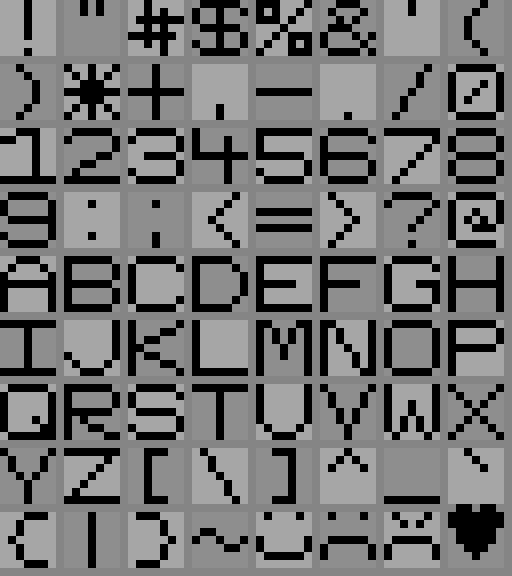
\includegraphics[width=\textwidth]{examples/workshop-mono-display}}
		\end{column}
	\end{columns}
\end{frame}

\begin{frame}
	\frametitle{Fonts on a Budget}
	\pause
	
	This is our strategy for embedding the fonts in C:
	
	\begin{itemize}
		\item Go through each 8x8 character, and for each of those characters read one 8 pixel column at a time.
		\item Convert that column into an 8-bit number; 1 = filled in pixel, 0 = blank pixel.
		\item Append this 8-bit number to a C string as one character / byte.
	\end{itemize}
	
	Not all characters can be represented by ASCII cleanly, so we'll need to use special conversion to represent them in the C string.
\end{frame}

\begin{frame}
	\frametitle{Fonts on a Budget}
	\pause
	
	\lstinputlisting[language=Python,firstline=1,lastline=24]{examples/bitmap-fonts.py}
	
	This is our script for converting bitmap font images to C strings.
\end{frame}

\begin{frame}
	\frametitle{Fonts on a Budget}
	\pause
	
	\lstinputlisting[language=Python,firstline=26,lastline=45]{examples/bitmap-fonts.py}
	
	This is our script for converting bitmap font images to C strings.
\end{frame}

\begin{frame}
	\frametitle{Fonts on a Budget}
	\pause
	
	\lstinputlisting[language=Python,firstline=47,lastline=51]{examples/bitmap-fonts.py}
	
	This is our script for converting bitmap font images to C strings.
\end{frame}

\begin{frame}[fragile]
	\frametitle{Fonts on a Budget}
	\pause
	
	Using this script we'll notice a problem:
	
	\begin{lstlisting}
$ ./bitmap-fonts.py | wc -c
1073\end{lstlisting}
	
	We have way too many characters. There are a number of ways we can deal with this:
	
	\begin{itemize}
		\footnotesize
		\item Each character has at least one column of spacing which will appear as `\texttt{\textbackslash0}', so we can skip this column entirely when encoding. \pause But we need to remember to add spacing between characters.
		\pause
		
		\item There are many other columns which are entirely blank which will also appear as `\texttt{\textbackslash0}'. We could replace `\texttt{\textbackslash0}' with another single character that doesn't appear in the C string (e.g. `w'), halving the size of each of these zeroes when embedded in the C string. \pause However, we need to remember to replace them with zeroes inside the code.
		\pause
		
		\item We could use a smaller font size such as 5x5. \pause But it would be harder to decode, since individual characters wouldn't fit neatly into bytes.
		\pause
		
		\item We could use some form of run-length encoding. \pause But it could make the C string actually larger depending on the way it's used, and would make decoding more complicated.
	\end{itemize}
\end{frame}

\begin{frame}[fragile]
	\frametitle{Fonts on a Budget}
	\pause
	
	This is a very tricky engineering problem. We need to consider how many characters we'll save by compressing various parts of the font vs. how many we'll gain with the compression code.
	\pause
	
	The first two options seem to be the most viable. We can even repeat the second option for other characters for more savings. We now have a much more reasonable count:
	\pause
	
	\begin{lstlisting}
$ ./bitmap-fonts.py | wc -c
807\end{lstlisting}
	\pause

	Now we can embed this font into our C code and start to use it.
\end{frame}

\section{Worked Examples}

\subsection{Worked Examples}

\begin{frame}
	\frametitle{Worked Examples}
	\pause
	
	We will now take some time to pick apart some finished examples.
	\pause
	
	\begin{itemize}
		\item My Discord status.
		\pause
		
		\item My Instagram bio.
		\pause
		
		\item The event banner code.
	\end{itemize}
\end{frame}

\end{document}
